\documentclass{article}
\usepackage[brazil]{babel}
\usepackage[utf8]{inputenc}
\usepackage{indentfirst}
\usepackage[T1]{fontenc}
\usepackage{gensymb}
\usepackage{graphicx}
\usepackage{etoolbox}
\usepackage[a4paper, left=20mm, right=20mm, top=20mm, bottom=20mm]{geometry}
\usepackage[colorlinks, urlcolor=blue, citecolor=red]{hyperref}



\begin{document}

\title{\textbf{Lógica Fuzzy}}
\author{
    Lucas Ribeiro Neis\\
     {\texttt{lucasrneis@gmail.com}}
     \and
     Vinícius Couto Biermann\\
      {\texttt{viniciusbiermann@hotmail.com}}
      \vspace{-50mm}
}
\date{Novembro 2016}

\maketitle

\section{Introdução}

O objetivo do trabalho é colocar em prática o conhecimento adquirido sobre lógica fuzzy. Para isso, foi proposto o desenvolvimento do controlador fuzzy para estacionar um caminhão de ré em uma doca. Foi fornecido um programa em java para fazer a simulação do caminhão e seus movimentos até a doca, calculando uma pontuação de acordo com a proximidade que o caminhão chegou da doca, o ângulo que estava, sendo próximo de 90\degree\ o melhor, e quantos passos foram necessários para chegar.


\section{Desenvolvimento}

Para o desenvolvimento, além do programa fornecido, foi utilizado a biblioteca \href{http://jfuzzylogic.sourceforge.net/}{JFuzzyLogic}. Com a biblioteca foi criado um arquivo em \textit{fuzzy control language} para representar as entradas, conjuntos fuzzy e regras para a realização de inferências.
Temos como entradas para o nosso sistema as posições $x$ e $y$ do caminhão na área e seu ângulo em relação ao eixo $x$. Após os processos da lógica, temos como saída um número que indica uma inclinação do volante para o próximo passo da simulação, podendo ser desde uma curva leve até o máximo de 30\degree\ permitido.
Nossa solução procura primeiro centralizar o caminhão enquanto já preparando-o para ficar com seu ângulo em 90\degree. Deste modo, quando o caminhão encontrar-se alinhado com a vaga, basta não alterar a direção e seguir em direção ao objetivo.

\subsection{Conjuntos Fuzzy}

A partir das entradas temos os seguintes conjuntos para a fuzzificação mostrados na figura \ref{fig01}.

O conjunto da entrada $x$ foi dividido em 6 partes para termos um melhor controle da posição do caminhão na área. Foi criado um termo para quando o caminhão está na área de alinhado com a doca em relação ao eixo $x$ e mais três termos para representar distâncias curtas, médias e longas para esquerda e direita da doca.

Para a entrada $y$, o que realmente precisamos saber é apenas se o caminhão está próximo demais da doca ou em uma distância boa para manobras tranquilas, assim temos apenas dois termos.

Por fim, o ângulo foi dividido em oito termos para melhor representar a real inclinação do veículo. Os ângulos de 0\degree\ e 360\degree\ são representados no mesmo termo, pois a inclinação é a mesma. O termo reflex representa os ângulos maiores que 180\degree\ e menores que 360\degree, onde o caminhão estará com a frente virada para baixo, mesmo que levemente. Os últimos seis ângulos foram criados em intervalos próximos para guiar de uma maneira mais precisa os movimentos do caminhão.


\subsection{Defuzzificação}

O método de defuzzificação utilizado foi o Centroide (Center of Gravity). Essa é a técnica mais comumente utilizada, nela temos uma única figura geométrica, obtida pela sobreposição dos conjuntos fuzzy escolhidos, que após o processo de fuzzificação são geralmente formados por trapezoides. É então calculado o centro de gravidade dessa nova figura e temos o seu valor $x$ como saída do processo de defuzzificação. O conjunto de termos da variável de saída é mostrado na figura \ref{fig02}.


\subsection{Regras}

Ao todo, foram criadas 44 regras. Levando em consideração todas as possibilidades, seriam possíveis 80 regras, no entanto, nossa abordagem toma alguns atalhos para casos onde não encontramos necessidade de lidar com certas variações. As regras podem ser encontradas no arquivo \texttt{truck.fcl} disponibilizado junto a este relatório.

Separamos, dentro do arquivo, por ângulos (primeiro quando o ângulo for \texttt{zero}, depois quando \texttt{acute} e assim por diante) para tornar melhor a visualização.

\begin{figure}[h!]
    \centering
    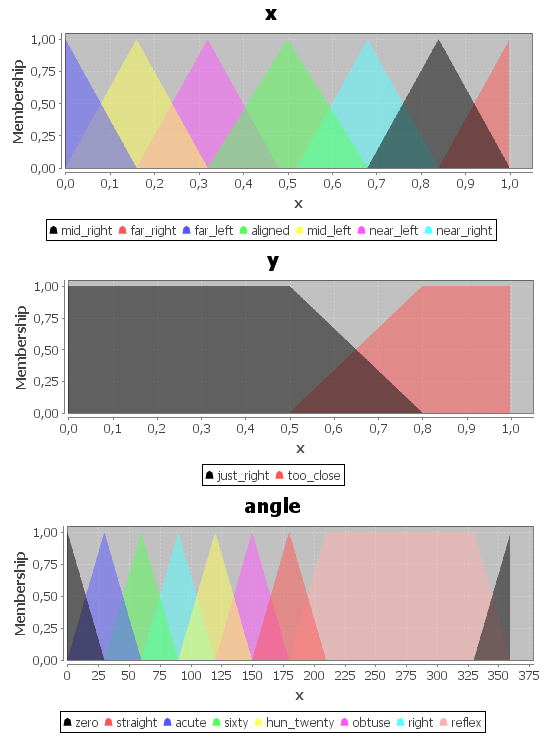
\includegraphics[scale=0.7]{figure1.png}
    \caption{Conjuntos fuzzy das posições nos eixos $x$ e $y$ e do ângulo do caminhão.}
    \label{fig01}
\end{figure}

\begin{figure}[h!]
    \centering
    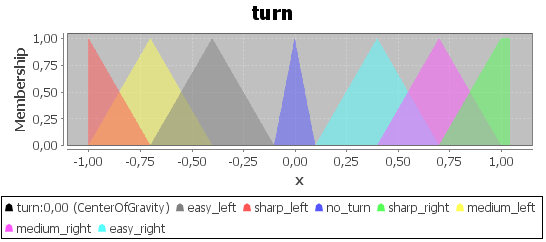
\includegraphics[scale=0.7]{figure2.png}
    \caption{Conjunto de defuzzificação.}
    \label{fig02}
\end{figure}

\pagebreak

\subsection{Dificuldades encontradas}

Apesar de ser o primeiro contato com fuzzy control language, foi uma tarefa rápida e fácil de aprender com os exemplos de uso da linguagem e manual encontrados no site oficial \cite{ref01}. O grande problema foi a escolha dos conjuntos, pois deviam fornecer uma boa simulação do mundo sem serem muito grandes ou muito pequenos.
O programa consegue estacionar o caminhão bem partindo de todas as posições que tiverem seu $y$ definido como \texttt{just\_right}, porém não de todas as posições com $y$ \texttt{too\_close}.
Com apenas as regras atuais, em uma posição muito perto, conseguimos resultados relativamente satisfatórios, com o caminhão parando na posição da doca, mas nem sempre em ângulos próximos à 90\degree.
O problema poderia ser corrigido com a adição de mais um termo no conjunto $y$, mas isso iria gerar várias novas regras para inferências com o novo valor e queríamos evitar o excesso de regras no trabalho.


\section*{Referência}

\patchcmd{\thebibliography}{\section*{\refname}}{}{}{}

\begin{thebibliography}{1}

  \bibitem{ref01} jFuzzyLogic. {\em Documentation \& a brief introduction to jFuzzylogic.} \href{jfuzzylogic.sourceforge.net/html/manual.html}{Link}
  
  \end{thebibliography}

\end{document}